\documentclass{article}

% Required packages for images and tight margins
\usepackage{graphicx}
\usepackage{geometry}

% Define very tight margins to maximize image area
\geometry{top=0.3in, bottom=0.3in, left=0.3in, right=0.3in}

\begin{document}

% No paragraph indentation for better alignment
\setlength{\parindent}{0pt}

% --- PAGE 1: dt=5 (Stacked tight) ---
\begin{figure}[h!]
    \centering
    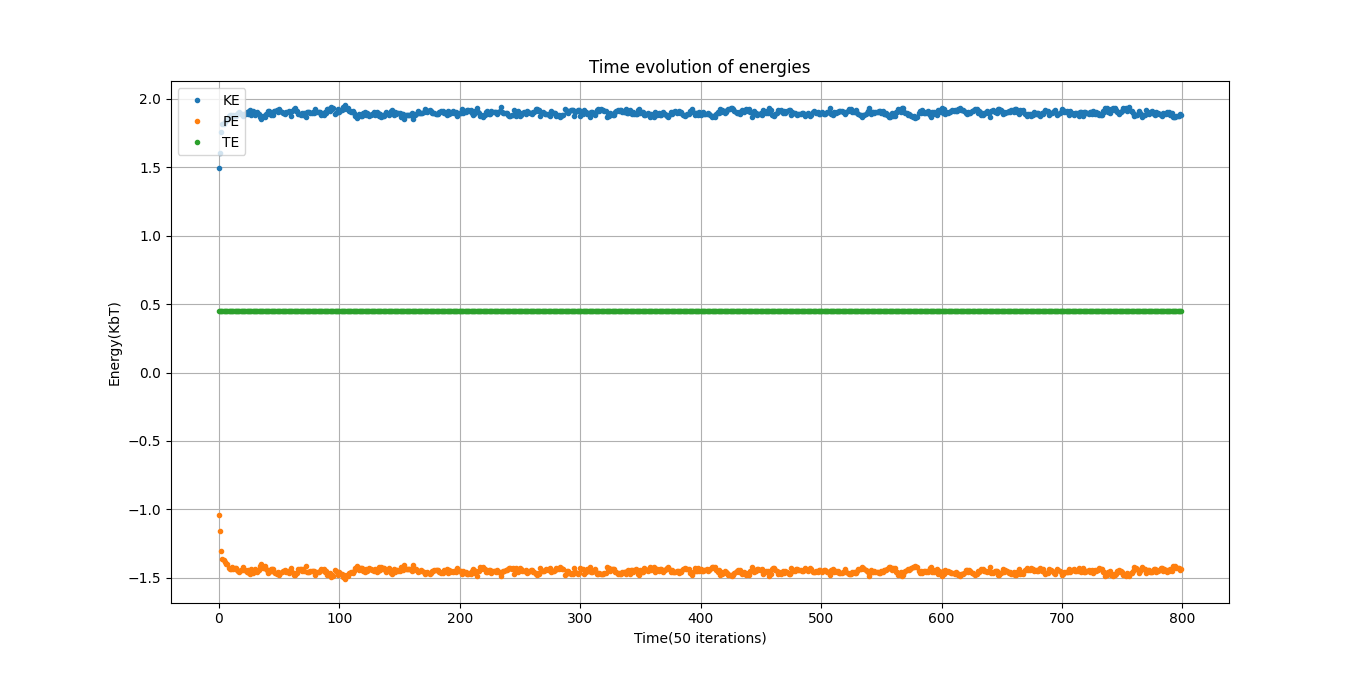
\includegraphics[width=0.92\textwidth]{Energy_evo_dt5.png}
    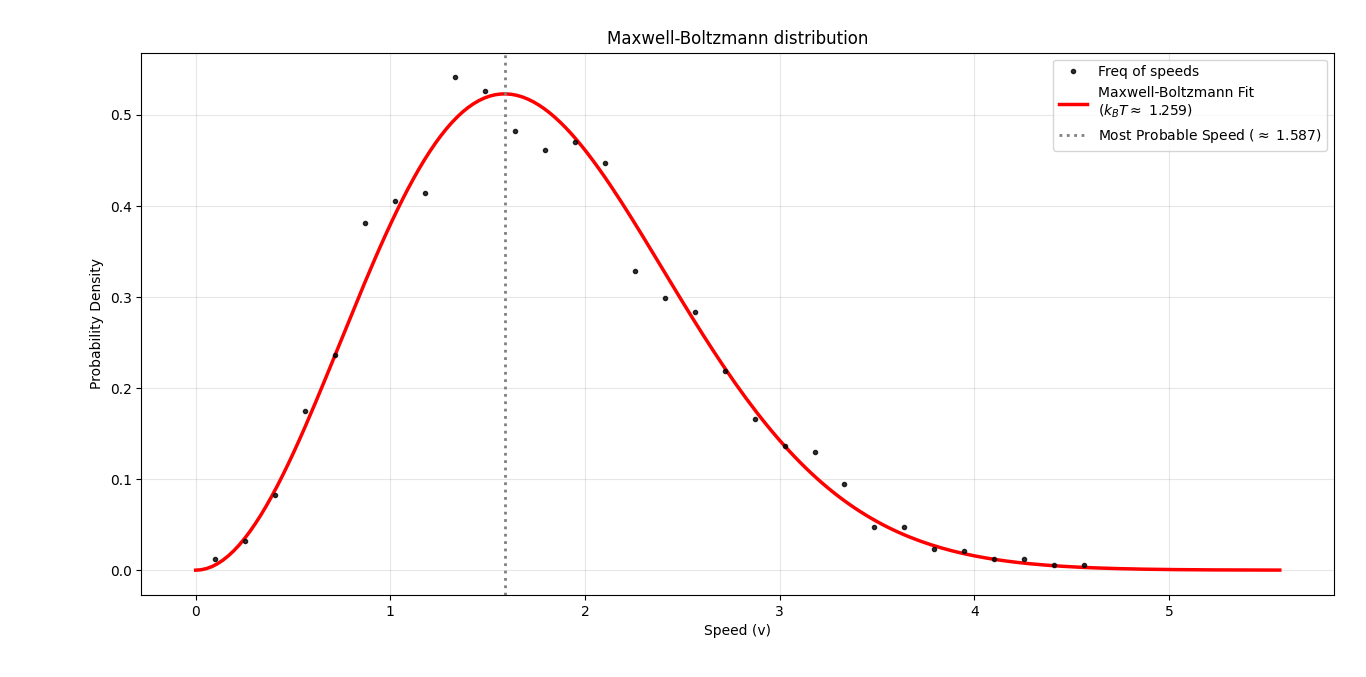
\includegraphics[width=0.92\textwidth]{mb_bare_dt5.png}
    \caption{dt=0.005 Energy Evolution and MB Distribution}
\end{figure}
\clearpage


% --- PAGE 2: dt=25 (Stacked tight) ---
\begin{figure}[h!]
    \centering
    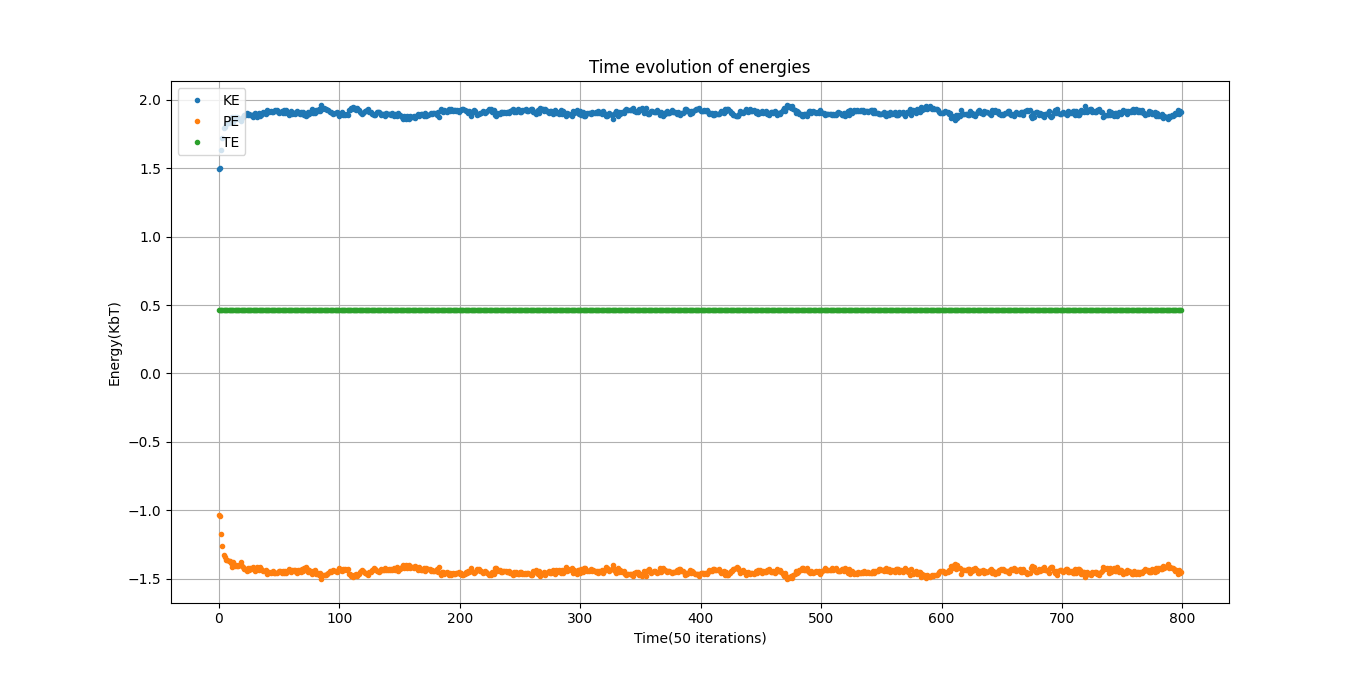
\includegraphics[width=0.92\textwidth]{Energy_evo_dt25.png}
    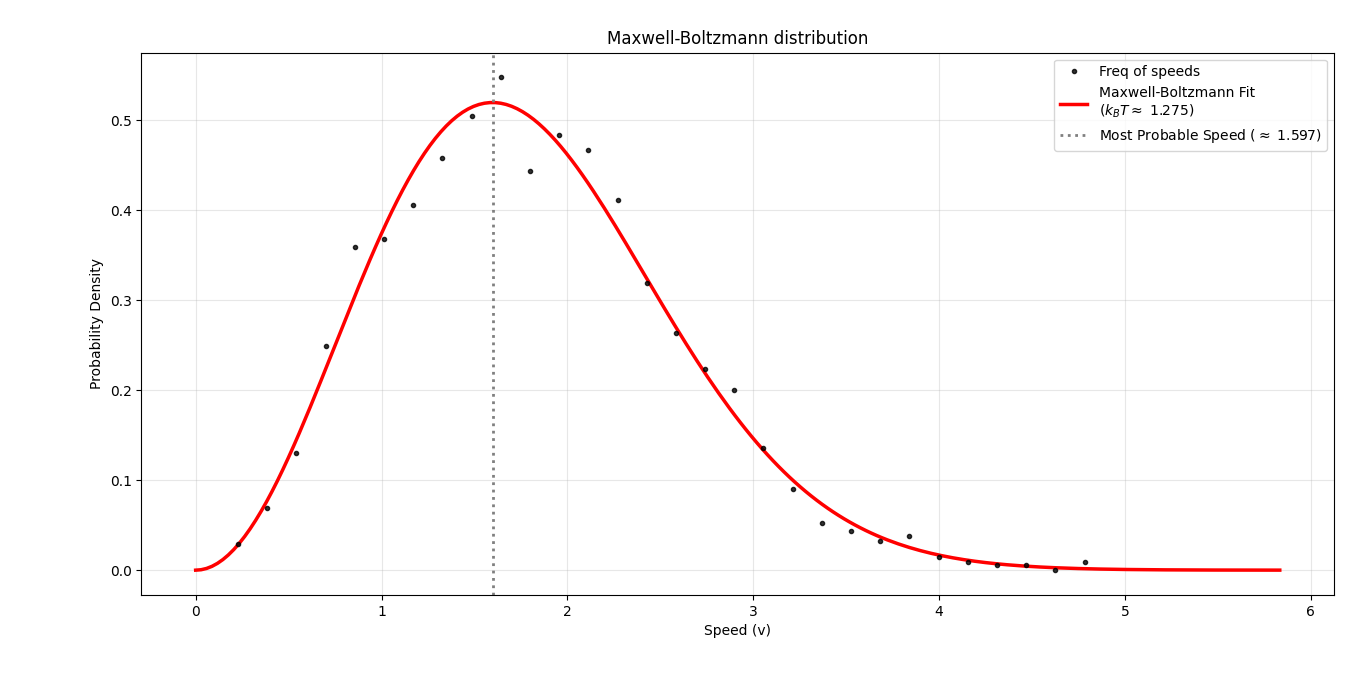
\includegraphics[width=0.92\textwidth]{mb_bare_dt25.png}
    \caption{dt=0.0025 Energy Evolution and MB Distribution}
\end{figure}
\clearpage


% --- PAGE 3: Energy Fluctuations (Stacked tight) ---
\begin{figure}[h!]
    \centering
    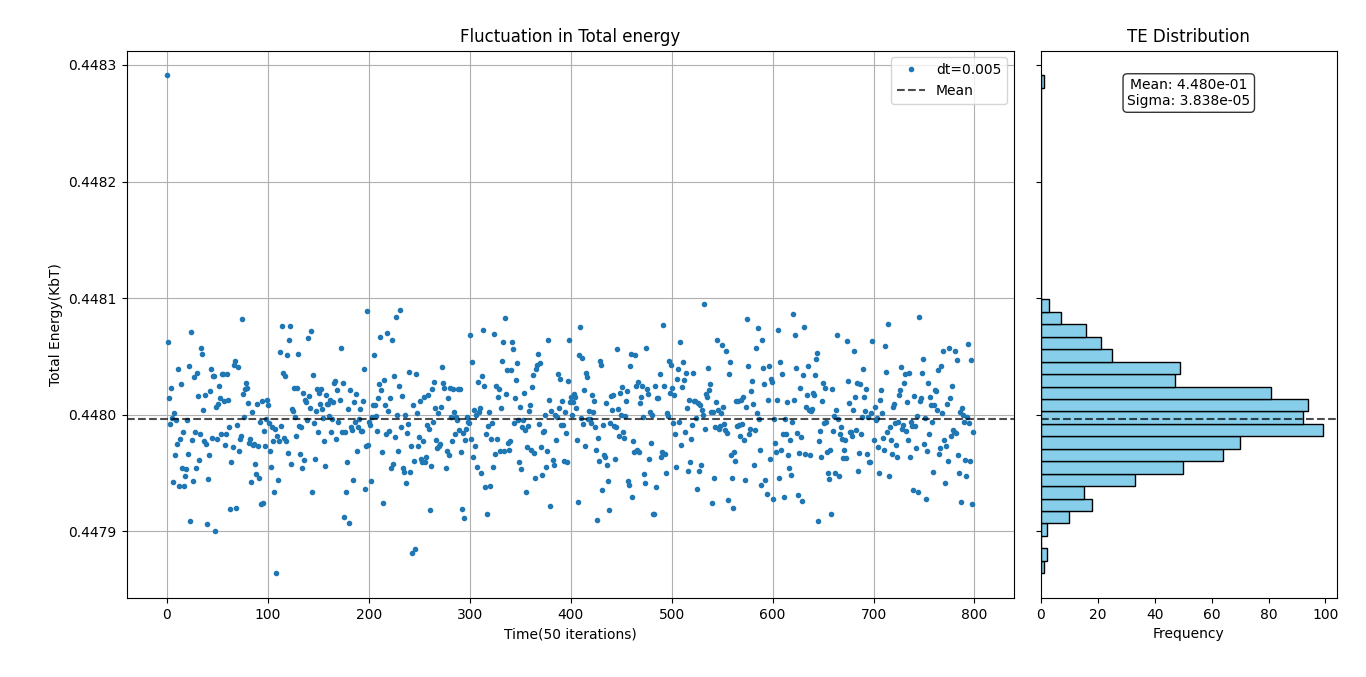
\includegraphics[width=0.92\textwidth]{Energy_fluc_dt5.png}
    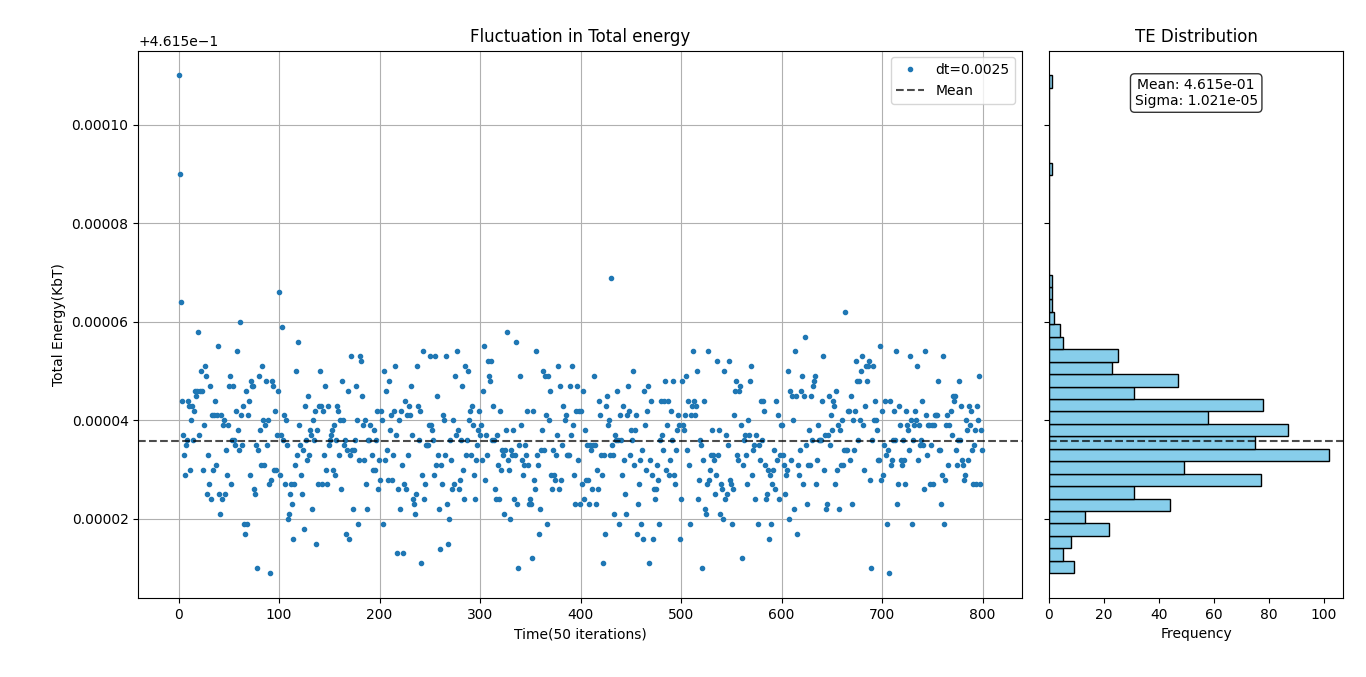
\includegraphics[width=0.92\textwidth]{Energy_fluc_dt25.png}
    \caption{Energy Fluctuations Comparison ($dt=0.005$ vs $dt=0.0025$)}
\end{figure}
\clearpage


% --- PAGE 4: Thermo Energy Evo (Stacked tight) ---
\begin{figure}[h!]
    \centering
    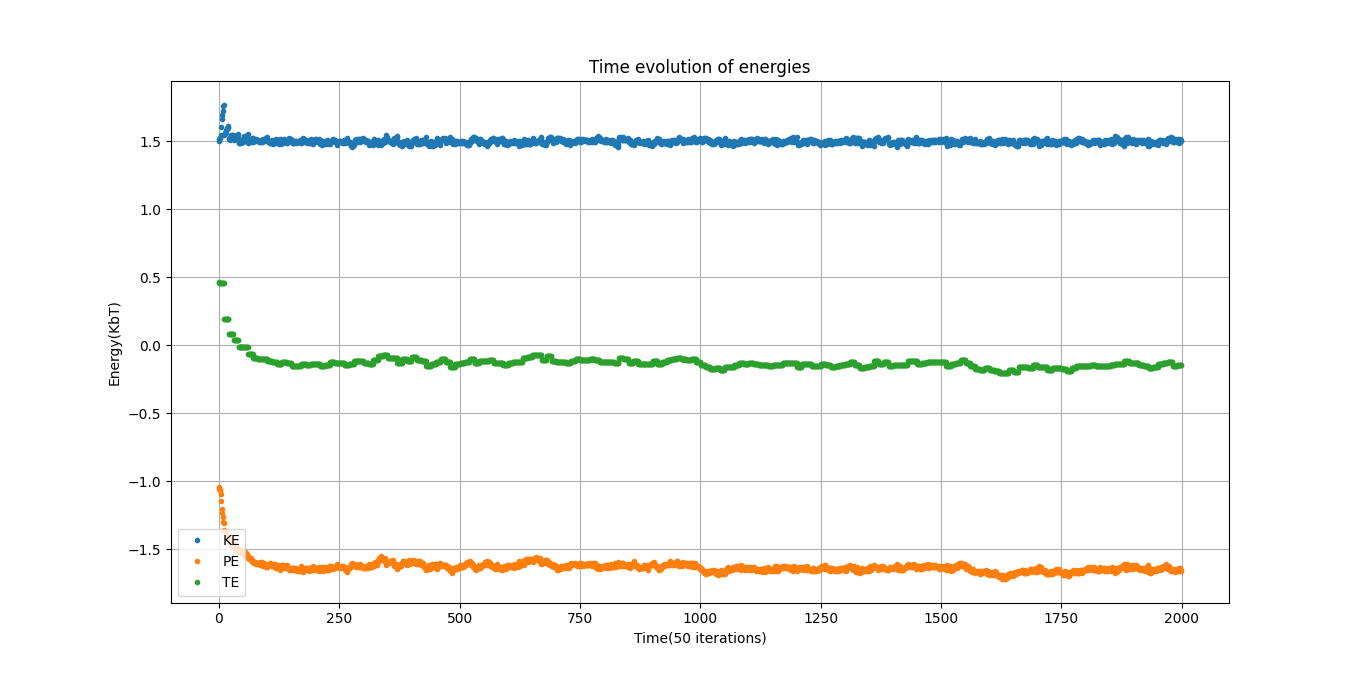
\includegraphics[width=0.92\textwidth]{Energy_evo_thermo.png}
    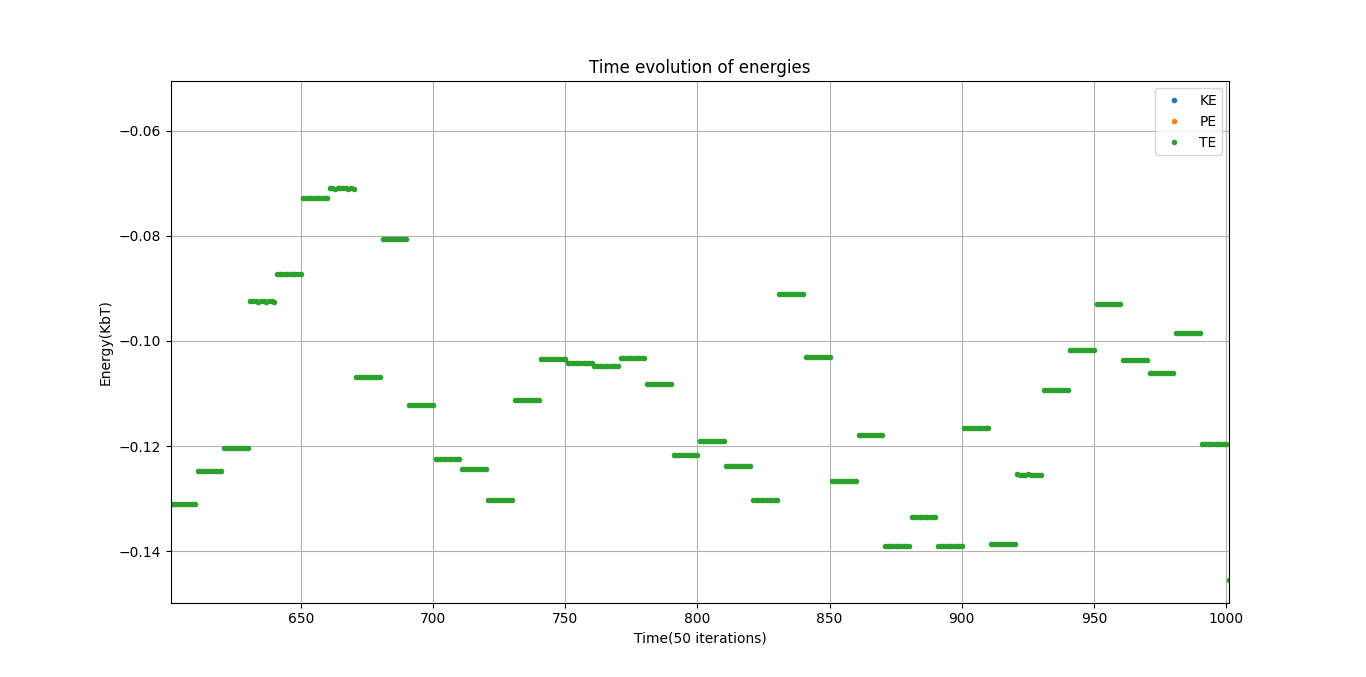
\includegraphics[width=0.92\textwidth]{Energy_evo_thermo_zoom.png}
    \caption{Energy Evolution with thermostat}
\end{figure}
\clearpage


% --- PAGE 5: Thermo MB (Single, maximized) ---
\begin{figure}[h!]
    \centering
    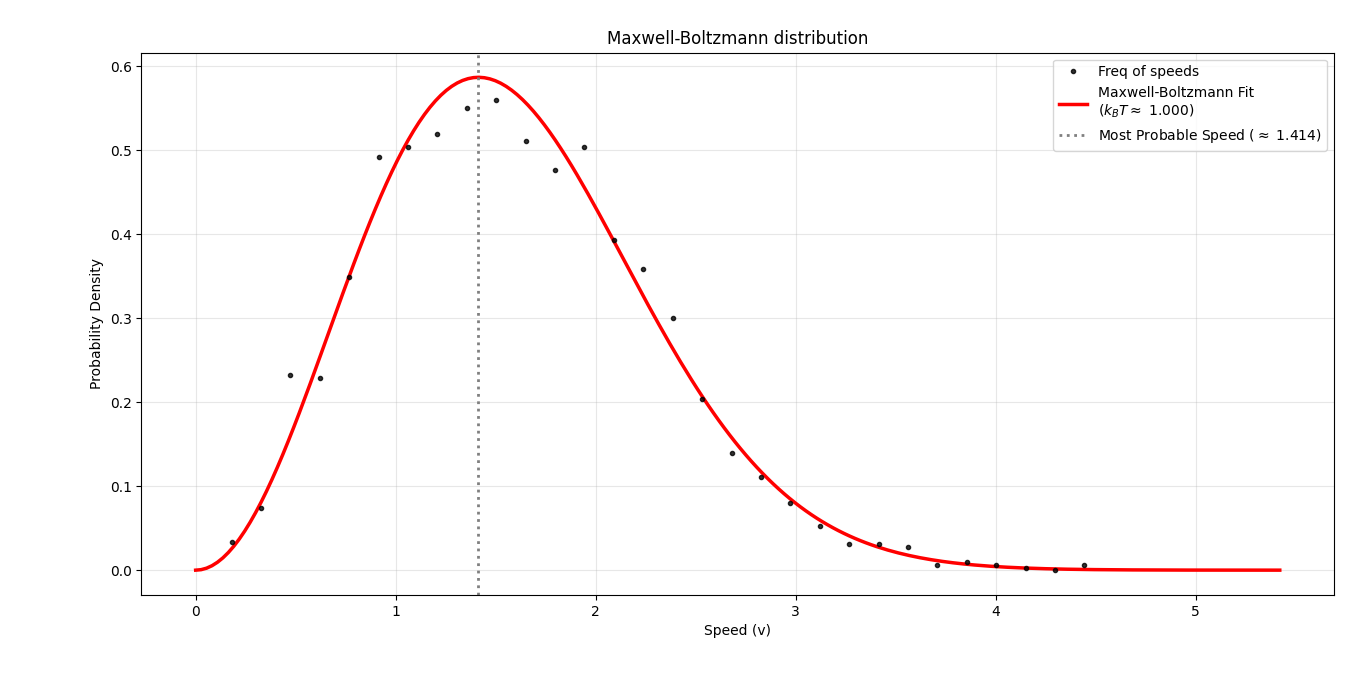
\includegraphics[width=0.98\textwidth]{mb_thermo.png}
    \caption{MB Distribution with thermostat}
\end{figure}
\clearpage


% --- PAGE 6: Energy Evo 1200, 2400, 3600 (Optimally Fitted 3-stack) ---
\begin{figure}[h!]
    \centering
    % Scaled width to fit 3 vertically
    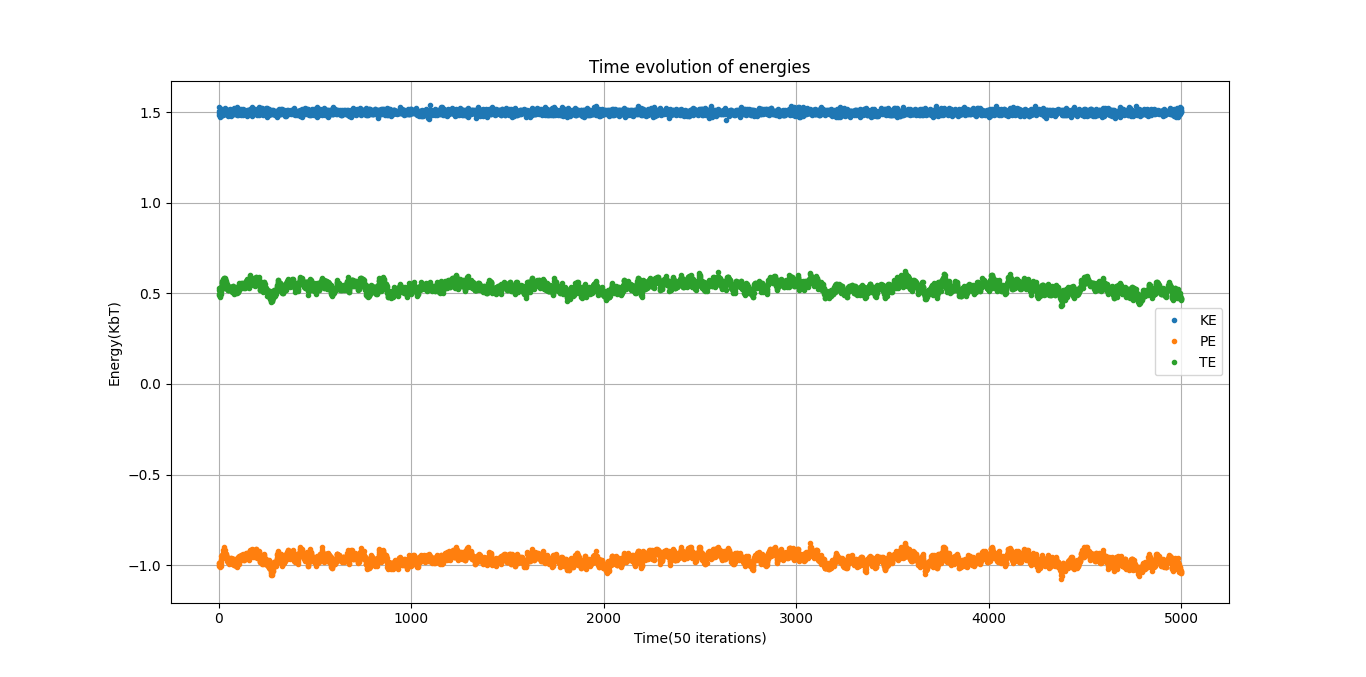
\includegraphics[width=0.55\textwidth]{Energy_evo_1200.png}
    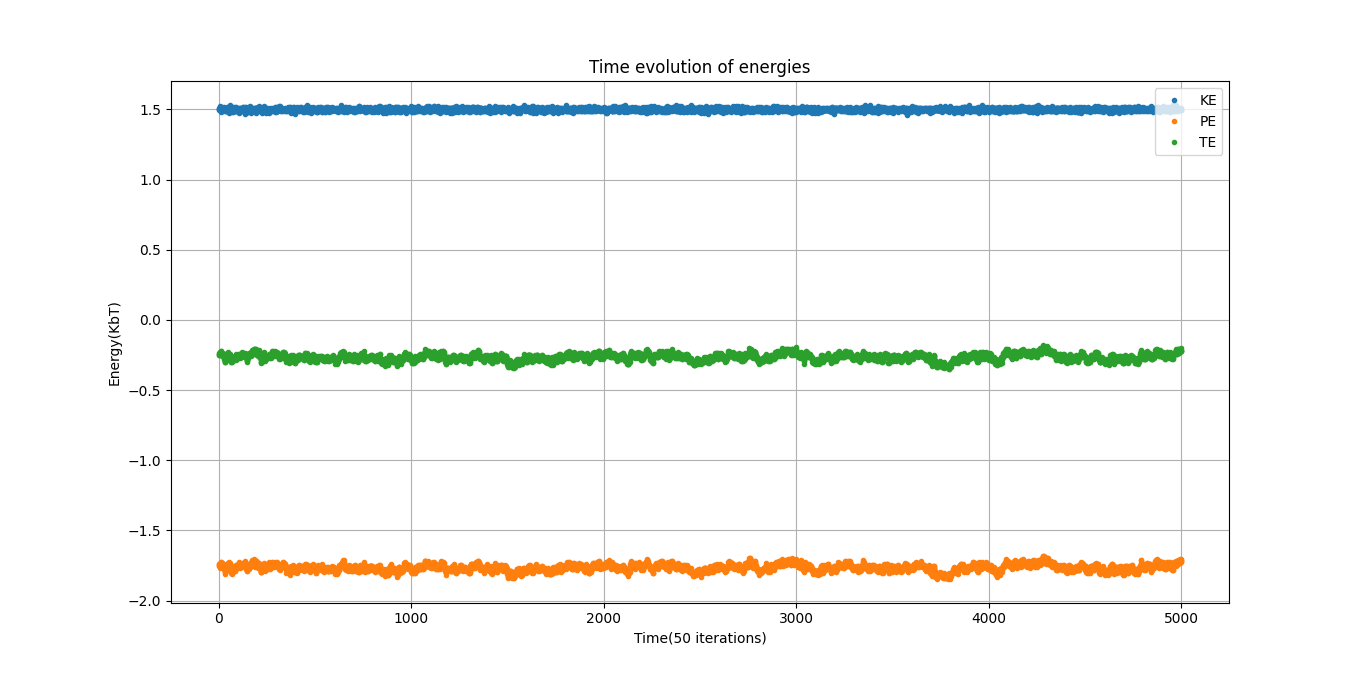
\includegraphics[width=0.55\textwidth]{Energy_evo_2400.png}
    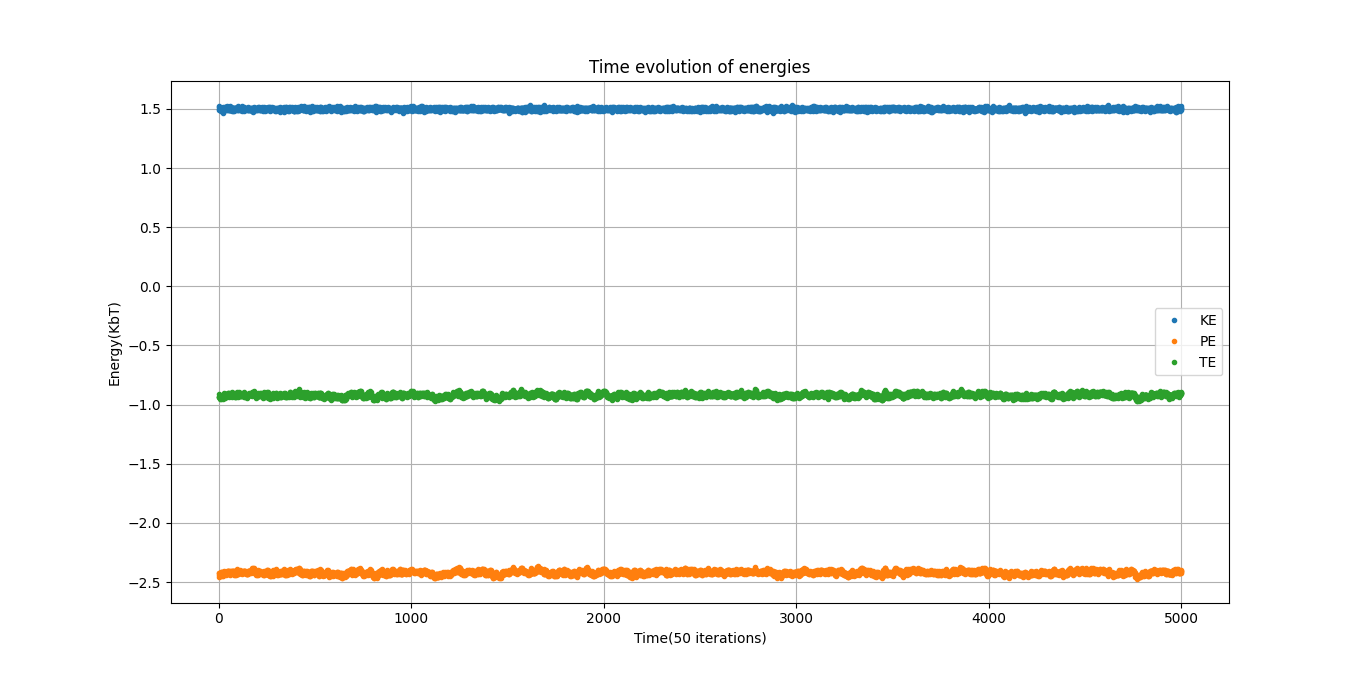
\includegraphics[width=0.55\textwidth]{Energy_evo_3600.png}
    \caption{Energy Evolution on varying no of part(1200, 2400, 3600)}
\end{figure}
\clearpage


% --- PAGE 7: 1200 pc and mb (Stacked tight) ---
\begin{figure}[h!]
    \centering
    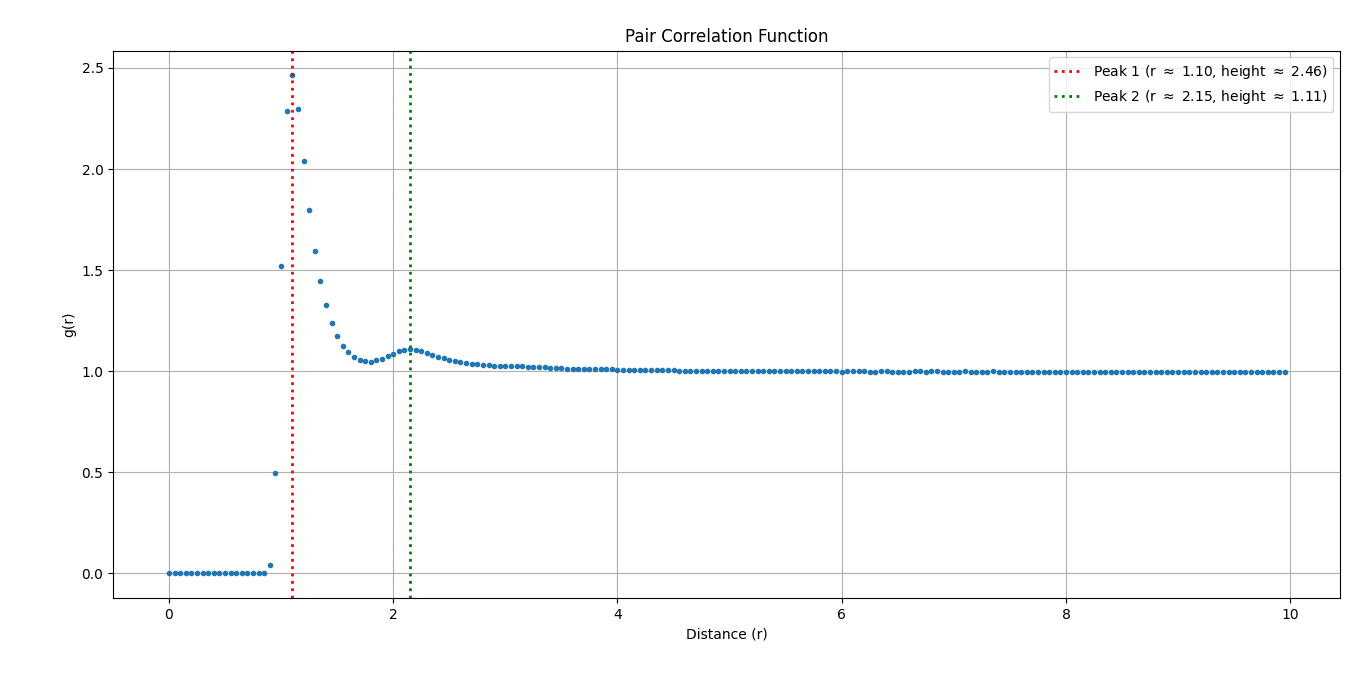
\includegraphics[width=0.92\textwidth]{pc_1200.png}
    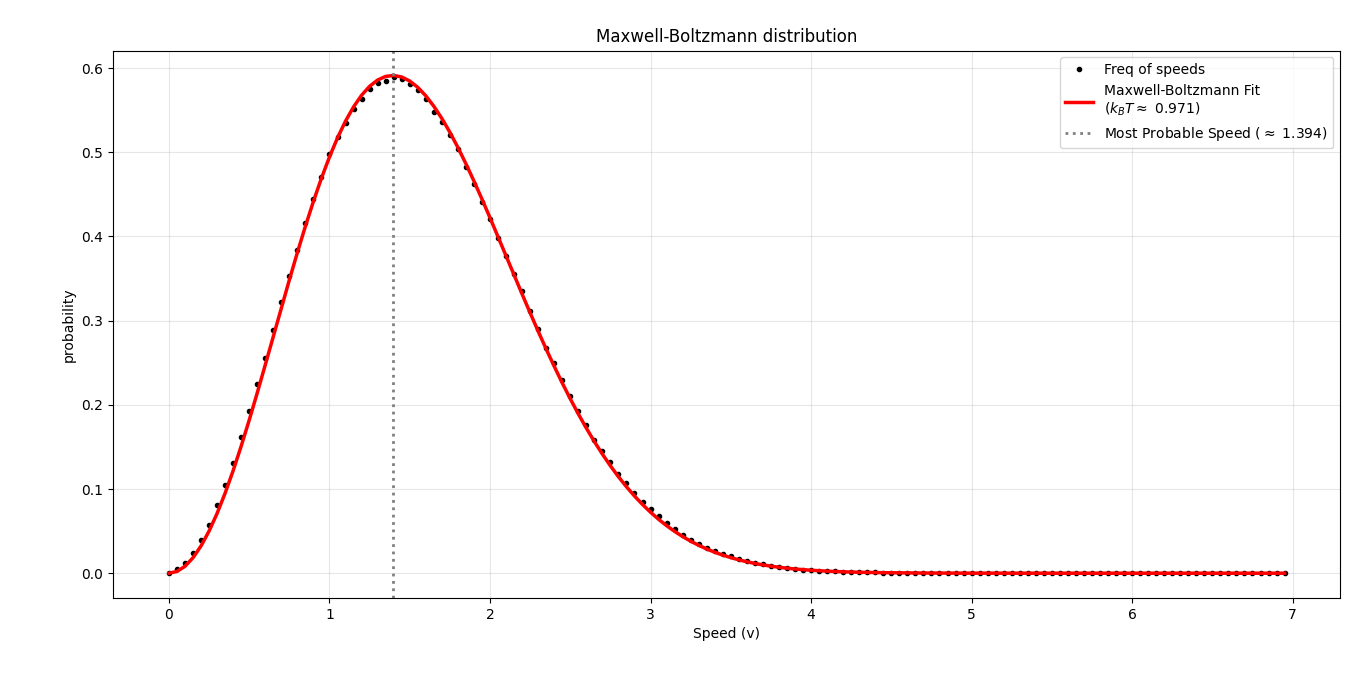
\includegraphics[width=0.92\textwidth]{mb_1200.png}
    \caption{1200 pair correlation and maxwell-boltzmann}
\end{figure}
\clearpage


% --- PAGE 8: 2400 pc and mb (Stacked tight) ---
\begin{figure}[h!]
    \centering
    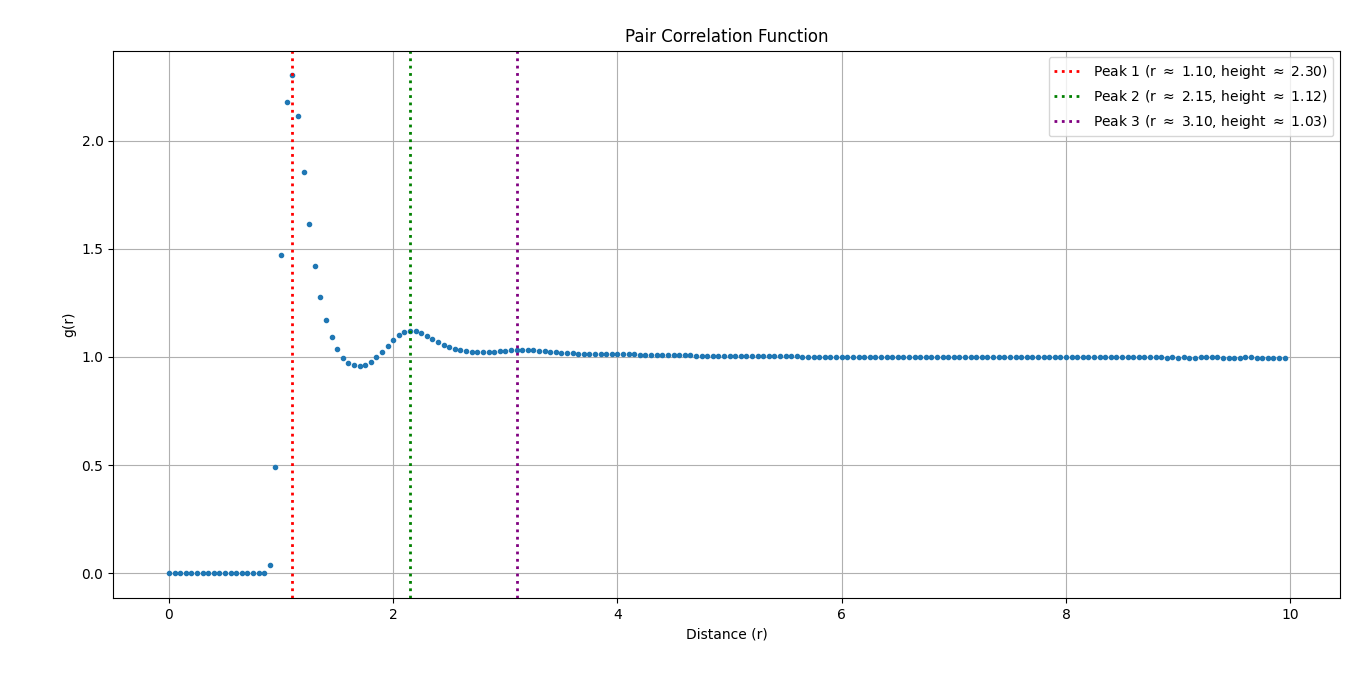
\includegraphics[width=0.92\textwidth]{pc_2400.png}
    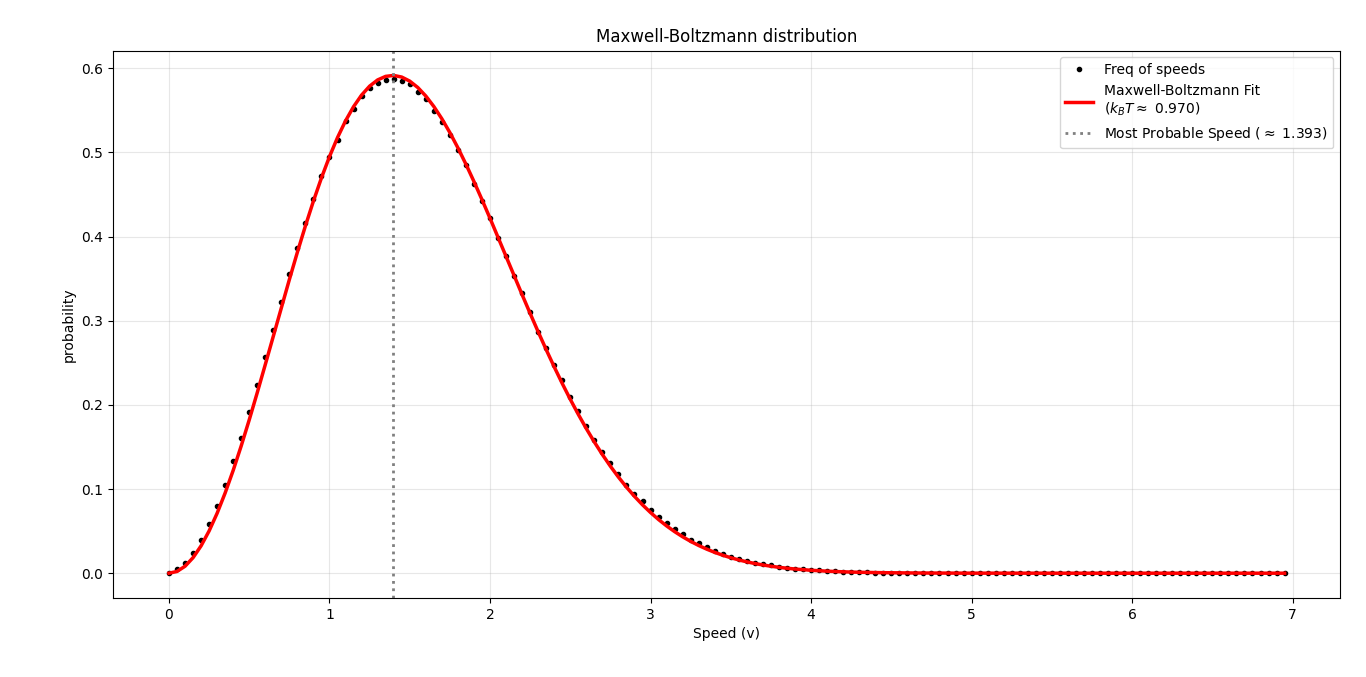
\includegraphics[width=0.92\textwidth]{mb_2400.png}
    \caption{2400 pair correlation and maxwell-boltzmann}
\end{figure}
\clearpage


% --- PAGE 9: 3600 pc and mb (Stacked tight) ---
\begin{figure}[h!]
    \centering
    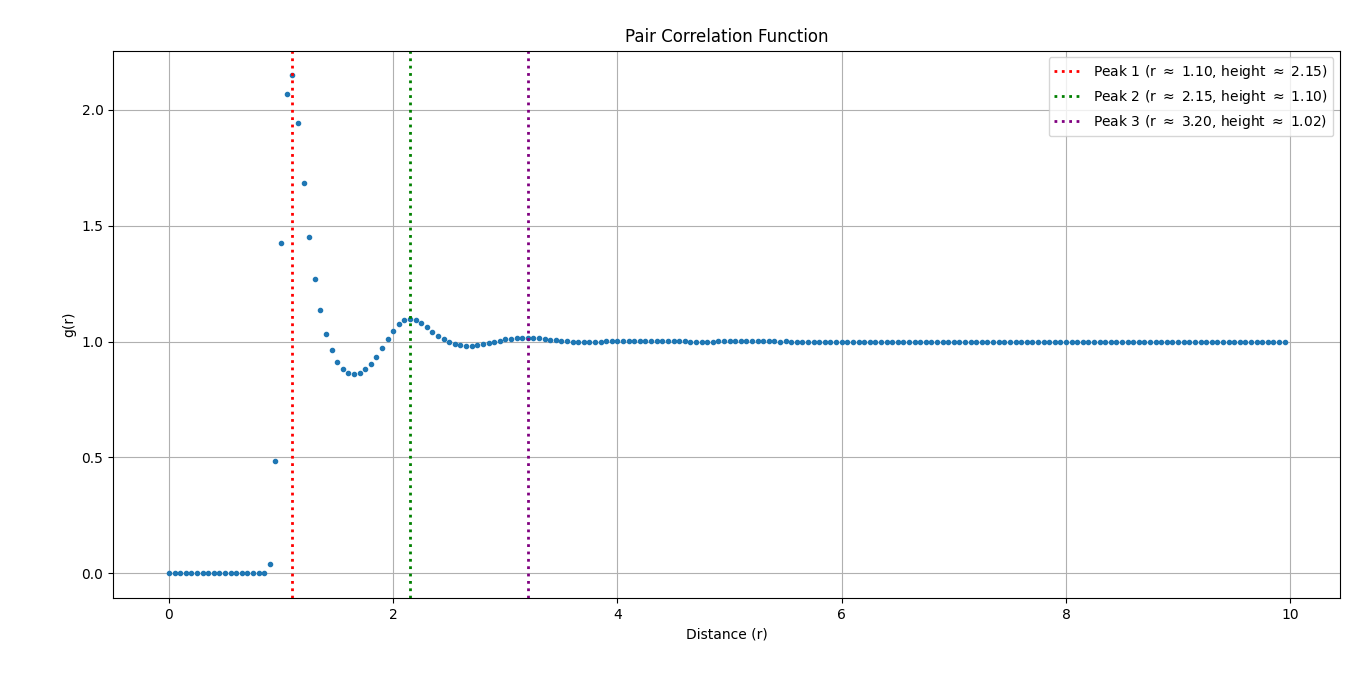
\includegraphics[width=0.92\textwidth]{pc_3600.png}
    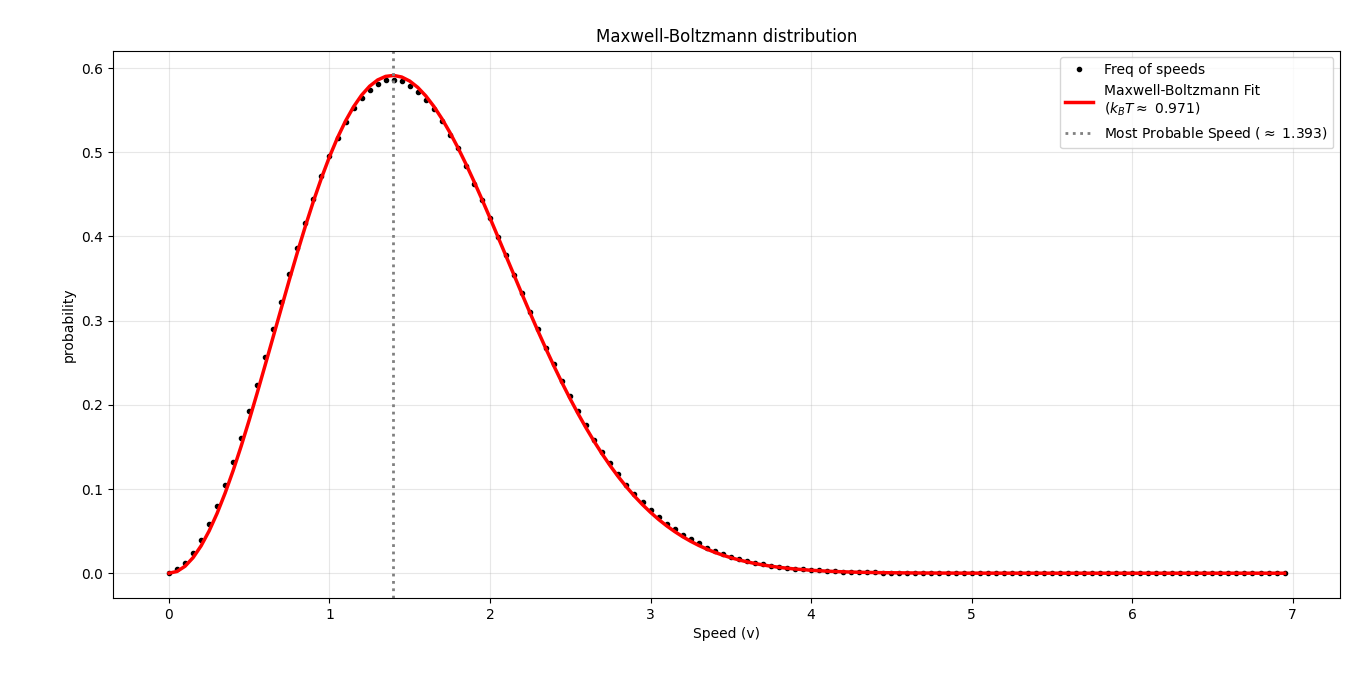
\includegraphics[width=0.92\textwidth]{mb_3600.png}
    \caption{3600 pair correlation and maxwell-boltzmann}
\end{figure}
\clearpage


% --- PAGE 10: PC Compare (Single, maximized) ---
\begin{figure}[h!]
    \centering
    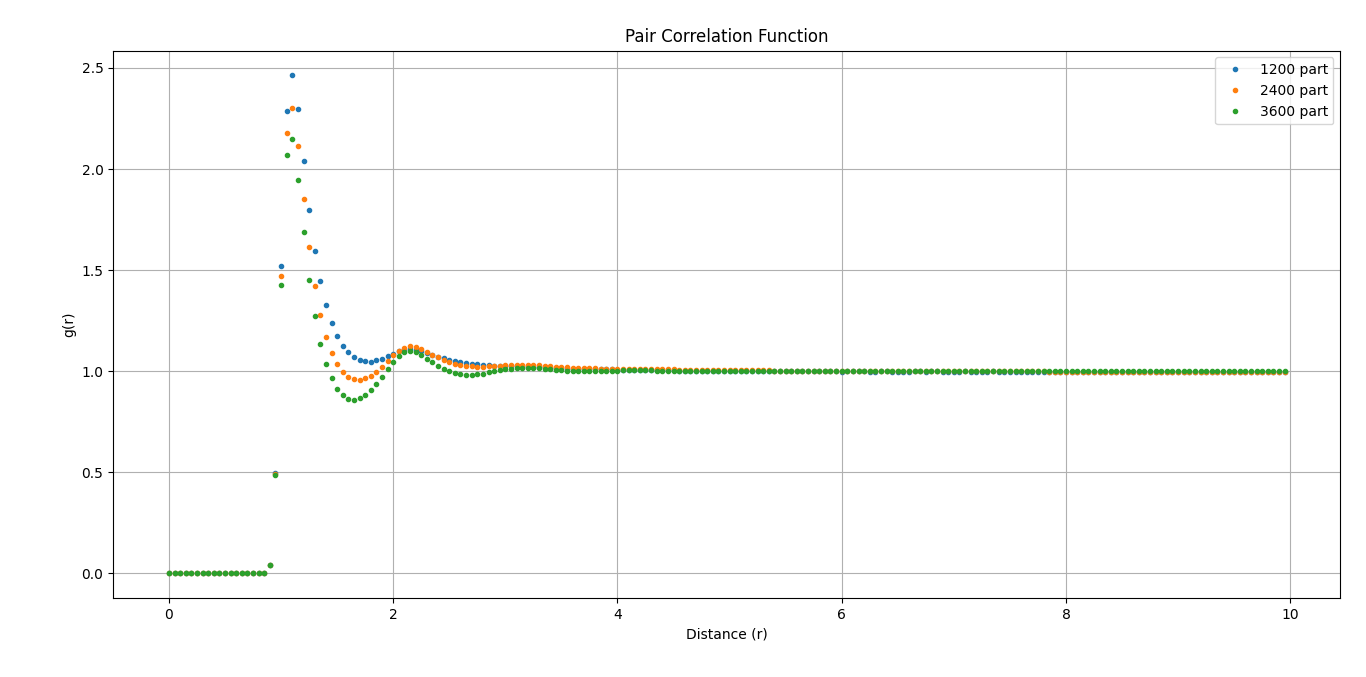
\includegraphics[width=0.98\textwidth]{pc_compare.png}
    \caption{Pair Correlation Comparison}
\end{figure}

\end{document}
